\documentclass[a4paper, oneside, 11pt, onecolumn]{article}
\usepackage[T1]{fontenc}
\usepackage{newtxtext,newtxmath}
\usepackage{graphicx}
\usepackage{subfigure}
\usepackage[round, comma, sort&compress, longnamesfirst]{natbib} 
% \usepackage[left=2cm,top=3cm,right=1.5cm,bottom=2cm,bindingoffset=0.5cm]{geometry}
\usepackage{enumerate}
\usepackage{fancyhdr}
\usepackage[title,titletoc,toc]{appendix}
\pagestyle{fancy}
\fancyhead{}
\fancyfoot{}
\fancyfoot[L]{\textit{running footer}}
 \fancyhead[L]{\textit{running title}}
\renewcommand{\headrulewidth}{0.8pt}
\renewcommand{\footrulewidth}{0.8pt}
\setlength\headheight{14pt}
\fancyfoot[RO] {\thepage}
\usepackage{authblk}
%%%%%%%%%%%%

\begin{document}

\title{Individual Differences Across Visual Search Tasks}

\author{A. D. F. Clarke, J. L. Irons, A. B. Leber and A. R. Hunt}
\affil{Aberdeen, Essex and Ohio}

\maketitle

\begin{abstract}
Some abstract goes here
\end{abstract}

%%%%%%%%%%%%%%%%%%%%%%%%%%%%
\section{Introduction}
%%%%%%%%%%%%%%%%%%%%%%%%%%%%


%%%%%%%%%%%%%%%%%%%%%%%%%%%%
\section{Methods}
%%%%%%%%%%%%%%%%%%%%%%%%%%%%


\subsection{Participants}
We aim to find 64 participants to volunteer to take part in this experiment. Participants will be students from the University of Aberdeen, and will be compenstate £x.xx for their time. Sample size was determined in part due to constraints with counter-balancing <expand>. 

\subsection{Materials and Procedures}

The study consists of three different paradigms from the visual search literature in which strong individual differences were found \citep{nowakowsak2017, irons-leber2016, kristjansson2014}.
{}
\subsubsection{A: Split-half array search}

\subsubsection{B: Attentional Control}

\subsubsection{C: Conjunction Foraging}

\subsection{Planned Analysis}

\subsubsection{A: Split-half array search}

In order to characterise an individual's behaviour in this task, we will compute the proportion of the first $n$ fixations that were on heterogeneous (difficult) side of the stimuli, over all target absent trials\footnote{Only take correct trials?}. \cite{nowakowsak2017} demonstrated a strong correlation between an this metric (for $n=5$) and reaction times ($r=$). However, a re-analysis of their data shows that an even stronger correlation is obtained with $n=3$ (see Figure \ref{fig:nowakowskaBestN})

\begin{figure}
\centering
\subfigure[][]{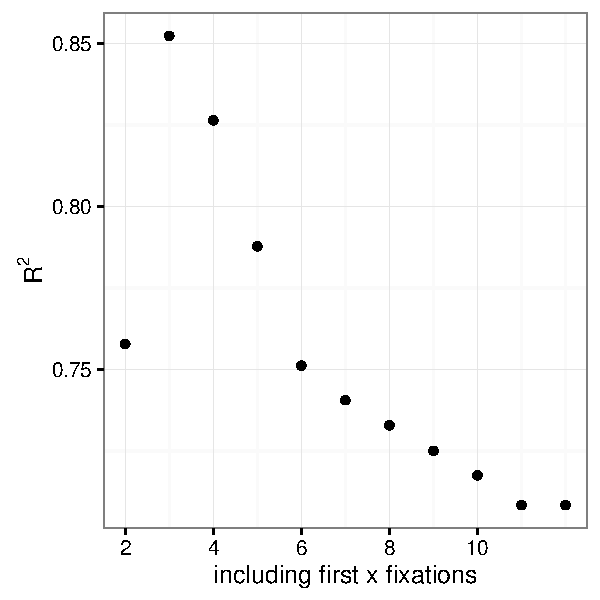
\includegraphics[width=6cm]{../NowakowskaClarkeHunt2017/scripts/r_by_nfix.pdf}}
\subfigure[][]{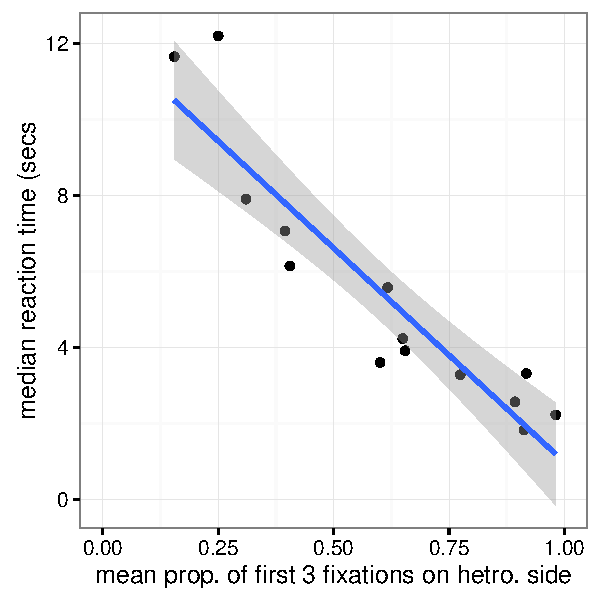
\includegraphics[width=6cm]{../NowakowskaClarkeHunt2017/scripts/best_r_scatter.pdf}}
\caption{Selecting the best $n$.}
\label{fig:nowakowskaBestN}
\end{figure}

\subsubsection{B: Attentional Control}

Following \cite{irons-leber2016}, individual differences will be characterized using two measures:\\
1) Proportion of optimal choices on plateaus. An optimal choice is defined as responding to whichever of the two target colours has the fewest items in the display. This will be based on correct plateau trials only. \\ 
2) Switching frequency. Switching is defined as responding to a different target color on trial $N$+1 than on trial $N$, and is presented as a proportion of the total number of trials (excluded incorrect trials, the trial after an incorrect trial, and the first trial of each block).\\
Both measures have been shown to correlate with overall RT in previous experiments (Proportion Optimal $r$=-.56, $p$<.001; Switch Frequency $r$=.45, $p$=.001; based on $N$=50 and using the same number of trials as in the current experiment). As additional validation, correlational analyses between both measures and RT will also be conducted in the current experiment.

\subsubsection{C: Conjunction Foraging}

Data analysis will follow \cite{kristjansson2014} and Johannesson et al. (2016). The main measure of interest will be the average run length per trial. A run is defined as a succession of one or more of the same target type which is followed and preceded by the other target type or no target. The average length is the average number of consecutive target selections per run. As with the other experiments, we will also measure the average response (time to select the final target on correct trials).

\subsubsection{}


\subsection{Exploratory Analysis}

We will carry out additional analysis, above and beyond what has been documented above, but the exact nature of this will be contingent on the nature of the results. Something like PCA may be interesting. 

%%%%%%%%%%%%%%%%%%%%%%%%%%%%
\section{Results}
%%%%%%%%%%%%%%%%%%%%%%%%%%%%

%%%%%%%%%%%%%%%%%%%%%%%%%%%%
\section{Discussion}
%%%%%%%%%%%%%%%%%%%%%%%%%%%%


%%%%%%%%%%%%%%%%%%%%%%%%%%%%
\begin{appendices}
\section{Hetero-Homo-geneous Array Search}
%%%%%%%%%%%%%%%%%%%%%%%%%%%%

%%%%%%%%%%%%%%%%%%%%%%%%%%%%
\section{Attentional Control Settings}
%%%%%%%%%%%%%%%%%%%%%%%%%%%%

%%%%%%%%%%%%%%%%%%%%%%%%%%%%
\section{Conjunction Foraging}
%%%%%%%%%%%%%%%%%%%%%%%%%%%%
\end{appendices}

\bibliographystyle{plainnat}
\bibliography{literature}

\end{document}


